%preamble
\documentclass{beamer} % use the beamer package for presentations
\usetheme{metropolis} % use the metropolis theme
\usepackage{wrapfig} % for text wrapping around figures

% used for formatting code blocks
\usepackage[most]{tcolorbox}
% \tcbuselibrary{skins}
% \newtcblisting{sh-input}{colback=black,colupper=white,colframe=black,
% listing only,listing options={style=tcblatex,language=sh},hbox,
% every listing line={\textcolor{cyan}{\small\ttfamily\bfseries\$}}}
% \newtcblisting{sh-output}{colback=black,colupper=white,colframe=black,
% listing only,listing options={style=tcblatex,language=sh},hbox,
% every listing line={\textcolor{white}{\tiny>}}}

% sets the location of the graphics directory
\graphicspath{ {./assets/images/} }

% title slide setup
\title{Methods in \\Research Software Engineering}
\date{6th May 2021}
\author{Dr David Wilby}
\institute{Research Software Engineering Team,\\ The University of Sheffield}
\titlegraphic{\vspace*{4cm}\hspace*{7cm}
\includegraphics[width=.3\textwidth]{RSE_logo_blackborder}}

% the main document
\begin{document}

  \begin{frame}
    \titlepage
  \end{frame}

  \begin{frame}{Outline}
    \begin{itemize}
      \item Introduction
      \item Academic Research
      \item Research Software Engineering
      \item Version Control
      \item GitHub (collaboration \& project management)
      \item Best Practice
      \begin{itemize}
        \item Documentation
        \item Commenting
        \item Code Style
        \item Testing
        \item Licenses
        \item Repository Organisation
      \end{itemize}
      \item Resources
      \item Nuggets of Wisdom
    \end{itemize}
  \end{frame}

  \begin{frame}{About Me}

    \begin{wrapfigure}{r}{0.3\textwidth}
        
\includegraphics[width=0.3\textwidth]{wilby}
    \end{wrapfigure}

    David Wilby

    \href{https://davidwilby.github.io/}{davidwilby.github.io/}

    \textbf{Who?}
    
    Research Software Engineer

    \textbf{Background}

    Optical Physics, Sensory Biology, Numerical Simulation, HPC

    \textbf{Interests}

    Python, Git, Matlab, Open Source, Web Apps, Research Impact

  \end{frame}

  \begin{frame}{Academic Research}
    \begin{itemize}
      \item Research papers
      \item Peer review
      \item Writing code
      \item Funding
      \item Impact
    \end{itemize}
    
  \end{frame}

  \begin{frame}{Research Software Engineering}
    \textbf{Goals}
    \begin{itemize}
      \item reproducibility
      \item transparency
      \item accountability
      \item exendability
      \item lifespan
      \item impact
    \end{itemize}

    \textbf{Methods}
    \begin{itemize}
      \item version control
      \item open source code
      \item reliable code
      \item documentation
    \end{itemize}
  \end{frame}




  \begin{frame}{Version Control}
    \begin{columns}
      \column{0.5\textwidth}
        How to use Git:
        \begin{itemize}
          \item \href{https://git-scm.com/}{Command Line Git 
\includegraphics[height=.05\textheight]{git}}
          \item \href{https://code.visualstudio.com/}{VS Code 
\includegraphics[height=.05\textheight]{vscode}}
          \item \href{https://www.gitkraken.com/}{GitKraken 
\includegraphics[height=.05\textheight]{gitkraken}}
          \item \href{https://gitforwindows.org/}{Git Bash 
\includegraphics[height=.07\textheight]{gitbash}}
          \item + many more...
        \end{itemize}


      \column{0.5\textwidth}
      Benefits of version control:
      \begin{itemize}
        \item try new ideas,
        \item confidence,
        \item ease of backing up (on remotes),
        \item 
      \end{itemize}
    \end{columns}
    
    \vspace{1cm}

    Learning resources:
    \begin{itemize}
      \item \textit{"oh sh** git"} - \href{https://wizardzines.com/zines/oh-shit-git/}{\underline{zine}}, or \href{https://ohshitgit.com/}{\underline{blog}}
    \end{itemize}

  \end{frame}

  \begin{frame}[fragile]{Git - useful commands}
    \begin{tcblisting}{beamer,colback=black,colupper=white,colframe=black,
      listing only,listing options={style=tcblatex,language=sh},hbox,
      every listing line={\textcolor{cyan}{\small\ttfamily\bfseries\$}}}
      git status
    \end{tcblisting}
    Show current branch, staged/tracked/untracked files, current status.
    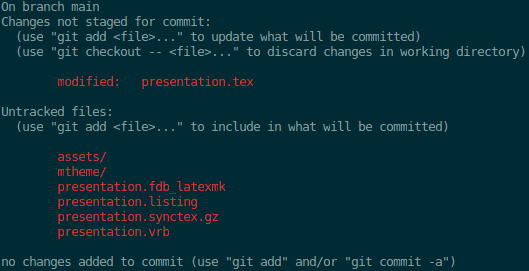
\includegraphics[height=.6\textheight]{git_status_output.png}
  \end{frame}

  \begin{frame}[fragile]
    'stash' your current unstaged changes.\newline
    \begin{tcblisting}{beamer,colback=black,colupper=white,colframe=black,
      listing only,listing options={style=tcblatex,language=sh},hbox,
      every listing line={\textcolor{cyan}{\small\ttfamily\bfseries\$}}}
      git stash
    \end{tcblisting}
    
    \begin{tcblisting}{beamer,colback=black,colupper=white,colframe=black,
      listing only,listing options={style=tcblatex,language=sh},hbox}
      Saved working directory and index state WIP on main: 3a158fc add some notes
    \end{tcblisting}

    Another couple to try:
    \begin{tcblisting}{beamer,colback=black,colupper=white,colframe=black,
      listing only,listing options={style=tcblatex,language=sh},hbox,
      every listing line={\textcolor{cyan}{\small\ttfamily\bfseries\$}}}
      git stash list
    \end{tcblisting}

    \begin{tcblisting}{beamer,colback=black,colupper=white,colframe=black,
      listing only,listing options={style=tcblatex,language=sh},hbox,
      every listing line={\textcolor{cyan}{\small\ttfamily\bfseries\$}}}
      git stash pop
    \end{tcblisting}
    
  \end{frame}

  \begin{frame}[fragile]
    \begin{tcblisting}{beamer,colback=black,colupper=white,colframe=black,
      listing only,listing options={style=tcblatex,language=sh},hbox,
      every listing line={\textcolor{cyan}{\small\ttfamily\bfseries\$}}}
    git log --decorate --all --oneline --graph
    \end{tcblisting}
    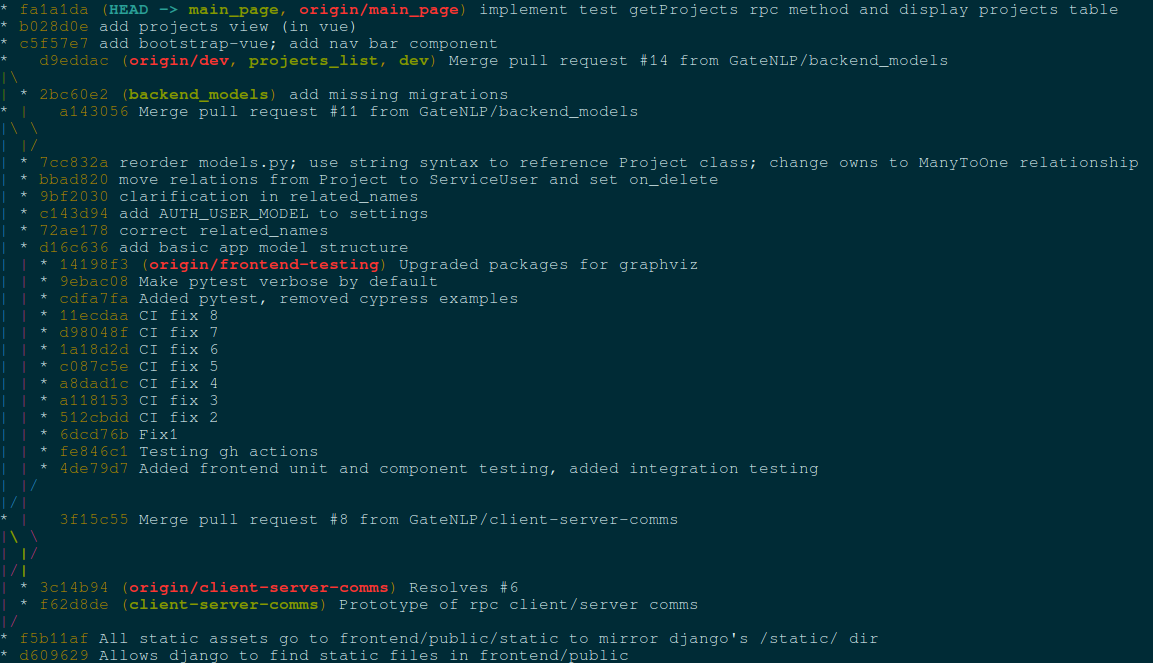
\includegraphics[height=.9\textheight]{git_log_tree_output.png}
  \end{frame}


  \begin{frame}{GitHub - collaboration}
    \begin{itemize}
      \item 
    \end{itemize}
  \end{frame}

  \begin{frame}{GitHub - project management}
  \end{frame}

  \begin{frame}{Best practice - documentation}
  \end{frame}

  \begin{frame}{Best practice - testing}
  \end{frame}

  \begin{frame}{Best practice - reproducibility}
  \end{frame}

  \begin{frame}{Best practice - code style}
  \end{frame}

  \begin{frame}{Best practice - environment management}
  \end{frame}

  \begin{frame}{Computing Resources at Sheffield}
  \end{frame}

  \begin{frame}{Summary}
    \begin{itemize}
      \item document, document, document
      \item keep things simple
      \item isolate environments
      \item version code \& data
    \end{itemize}
  \end{frame}

\end{document}
